\documentclass{article}
\usepackage[utf8]{inputenc}
\usepackage{setspace}
\usepackage{graphicx}
\usepackage{epstopdf}
\usepackage[margin=0.75in]{geometry}

\title{Management and Organizational Practices Survey in Colombia}
\author{Leonardo Iacovone,
Javier Fernandez}
\date{\today}

\begin{document}

\maketitle

\section{Abstract}
\doublespacing
Matching the Innovation and Technology Survey EDIT 2017-2018 (acronym in Spanish) with Annual Manufacturing Survey 2018 (EAM), we analyze the relationship between the performance and management at firm level for Colombia in 2018. The management is a driver of variation in the productivity, the investment on research, development and innovation (RDi) and intellectual property registers. Also, we find a statistically significant relationship between the management competence and the number of export destinations, products and export revenues,mainly in products with greater complexity. Finally, these findings are discussed, highlighting the high profitability for companies to improve their capacities and their public policy implications.

\section{Introduction}

\section{Measuring Management}

The Management and Organizational Practices Survey was incorporated for the first time in EDIT 2017 2018 (Innovation and Technology Survey in Colombia for Manufacturing Sector) and published with anonymous data on the website of the Colombian Institute of Statistics (DANE). The EDIT included 16 management
questions with two basic areas, which are supported on the idea of the continuous improvement. For our regressions, we aggregate those 16 questions into a single measure, which is called the management score. This score is the unweighted average, where the answer to each question is measured on a scale from 0 to 1.

For our regressions, we aggregate those 16 questions into a single measure, which is called the management score. This score is the unweighted average, where the answer to each question is measured on a scale from 0 to 1, where o is the worst option and 1 the best. Table 1 presents the descriptive statistics of the successful merge between EDIT and EAM, and some characteristics at the signature level. In cases where the firm has
more than one establishment, the information is added. For our analysis, we use data with at least eleven non-missing responses to the management questions that also have positive values for outcomes and inputs
of the firm.

According to Bloom(2019) the average U.S Management score (1-16 questions) is 0.615, the non-incentives (1-8) is 0.643 and the incentives (9-16) is 0.583.The following histogram shows the distribution for management score (16 questions) for Colombia and the United States, using the merge between EDIT and EAM with 6,034 observations. It plots the overlapping histogram of firm management scores for Colombia (2018) and the United States (2010) according to Bloom (2019). While the Colombian management score (from 1 to 16 questions) was 0.37, for the U.S was 0.61, which implies that the distribution of Colombia is skewed to the left compared to the United States.

The histogram below shows the distribution for management score (16 questions). As you can see, the distribution is skewed to the left, where the total number of observations is 7,529 in EDIT. This histogram includes all observations with at least 11 non-missing responses to management questions.

\begin{figure}
	\caption{Histogram Colombia - The United States}
    \centering
	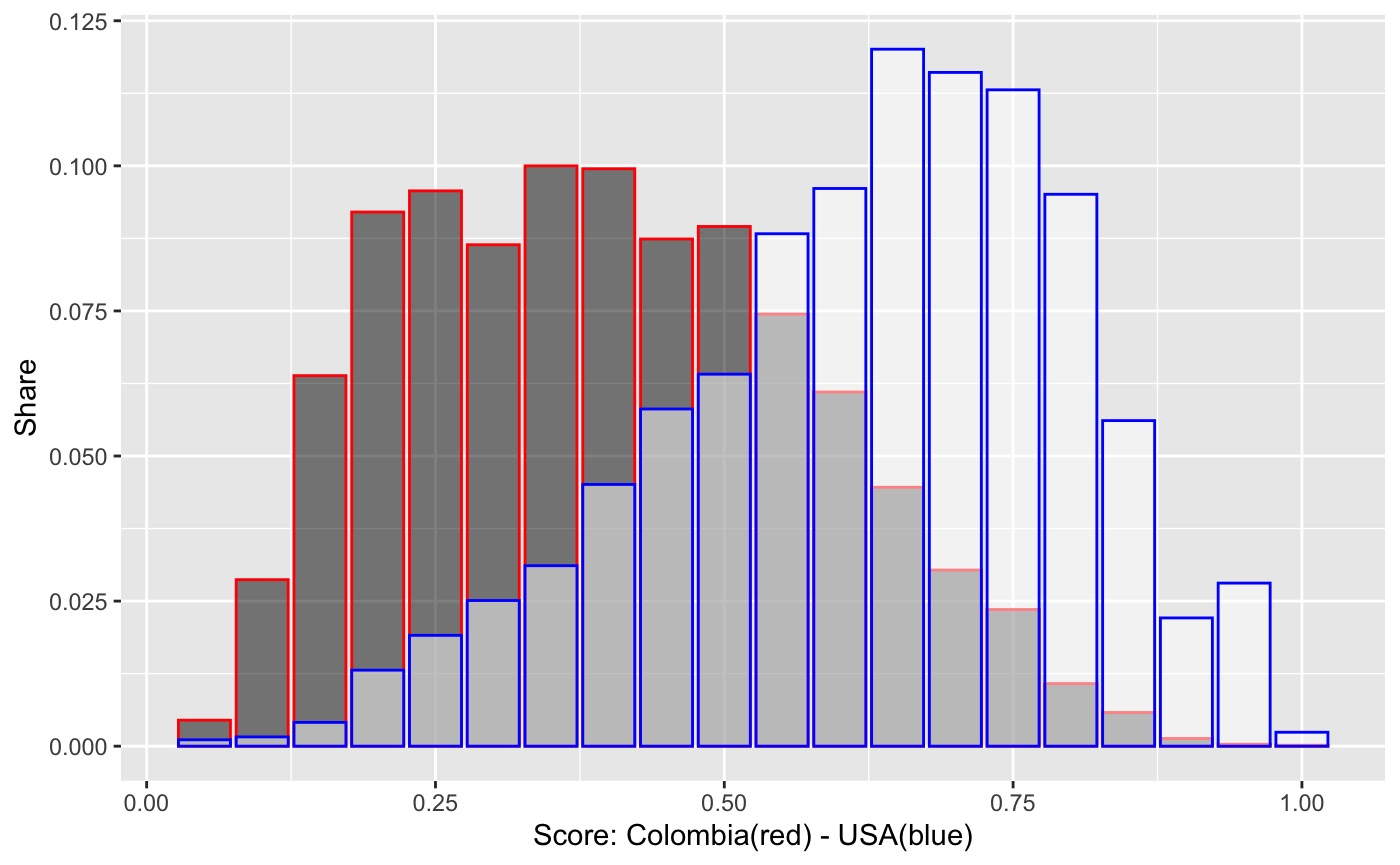
\includegraphics[scale = 0.25]{Images/Histogram.jpg}
\end{figure}
\doublespacing

Figure 2 shows a positive correlation between Management score with the average of value added per employee, exports, investment on research, development and innovation, intellectual registers and wage per employee.


\begin{figure}
    \caption{Performance and Structured Management}
    \centering
    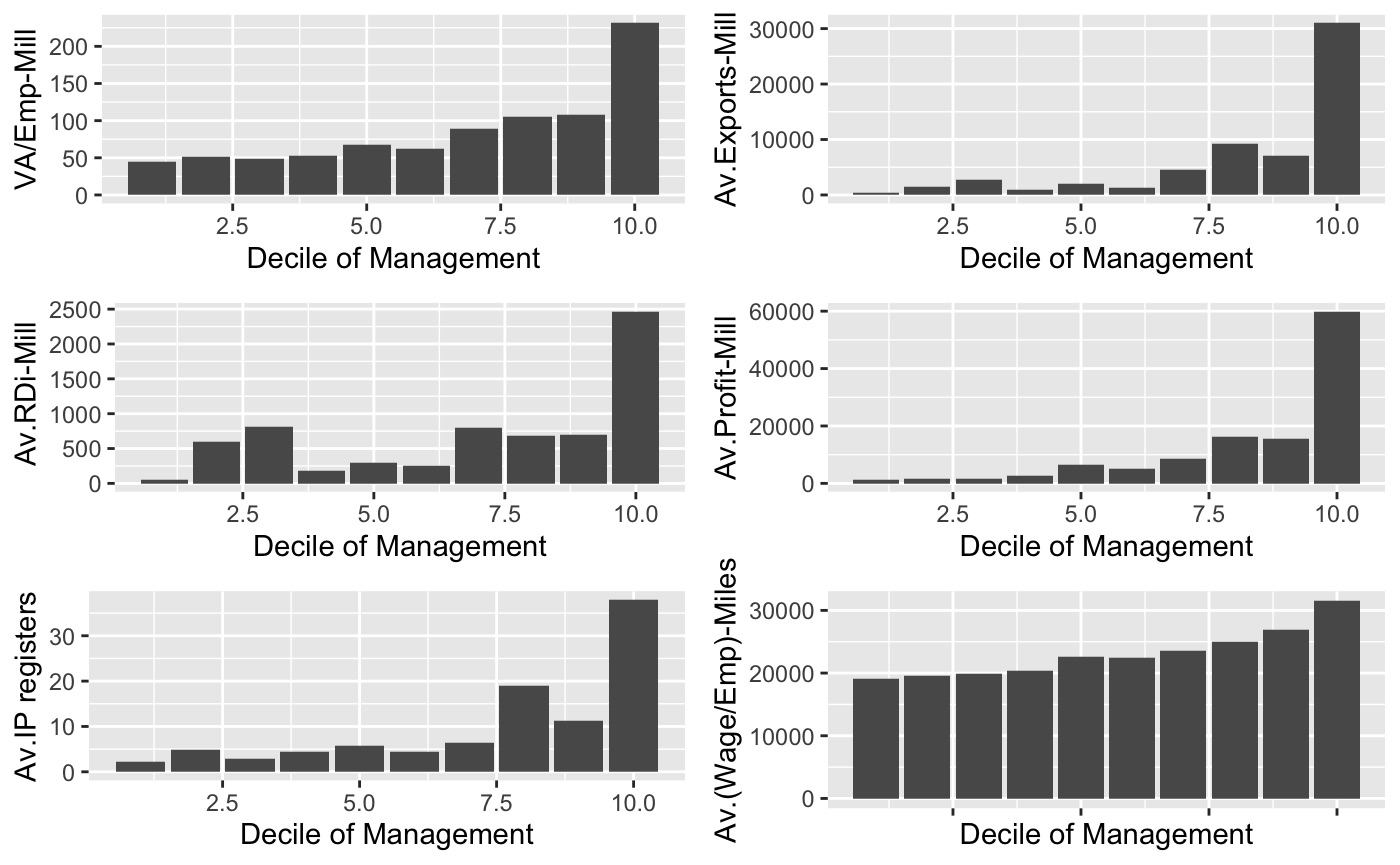
\includegraphics[scale = 0.25]{Images/Deciles.jpg}
\end{figure}

\doublespacing

\section{Management and Performance}

We divide the performance into four groups of dependent variables: a) productivity: production, sales, value added, total factor productivity b) Innovation: investment on research, development and innovation (RDi) and intellectual properties register c) market competition: management score d) trade: exports, imports, number of products sold abroad, destinations, destination-product pairs, exports over product destination pairs and exports at top destination-product.

We investigate whether management competence is correlated with those measures of performance. We do not attribute a causal interpretation to the results, instead, it replicates the most of regression from Bloom (2019) and Manova (2020), which allows compare coefficients between Colombia and the United States.

\subsection{Data}

\subsection{Empirical Strategy}

\subsection{Findings}


\subsubsection{Summary Statistics}


\begin{table}[!htbp] \centering 
  \caption{Descriptive Statistics} 
  \label{} 
\begin{tabular}{@{\extracolsep{5pt}}lccccccc} 
\\[-1.8ex]\hline 
\hline \\[-1.8ex] 
Statistic & \multicolumn{1}{c}{N} & \multicolumn{1}{c}{Mean} & \multicolumn{1}{c}{St. Dev.} & \multicolumn{1}{c}{Min} & \multicolumn{1}{c}{Pctl(25)} & \multicolumn{1}{c}{Pctl(75)} & \multicolumn{1}{c}{Max} \\ 
\hline \\[-1.8ex] 
Management (1-16) & 6,034 & 0.376 & 0.176 & 0.026 & 0.231 & 0.504 & 0.958 \\ 
No Incentives (1-8) & 6,034 & 0.555 & 0.198 & 0.056 & 0.402 & 0.701 & 1.000 \\ 
Incentives (9-16) & 6,034 & 0.222 & 0.191 & 0.000 & 0.071 & 0.357 & 0.952 \\ 
Size(Firm employment) & 6,034 & 125.502 & 254.973 & 0 & 18 & 117 & 4,181 \\ 
Multiplant & 6,034 & 0.044 & 0.206 & 0 & 0 & 0 & 1 \\ 
Destinations & 2,076 & 7.730 & 10.809 & 1.000 & 1.000 & 9.000 & 110.000 \\ 
Products & 2,076 & 9.124 & 18.858 & 1.000 & 2.000 & 9.000 & 340.000 \\ 
Dest-Prod & 2,076 & 34.251 & 126.804 & 1.000 & 2.000 & 25.000 & 2,795.000 \\ 
Exporters & 6,030 & 0.357 & 0.479 & 0.000 & 0.000 & 1.000 & 1.000 \\ 
Import/Input & 6,030 & 0.078 & 0.221 & 0.000 & 0.000 & 0.001 & 8.591 \\ 
Export/Sales & 6,030 & 0.070 & 0.168 & 0.000 & 0.000 & 0.038 & 1.000 \\ 
\hline \\[-1.8ex] 
\multicolumn{8}{l}{Note:The management score is the unweighted average of the score for each of the 16 questions, where} \\ 
\multicolumn{8}{l}{each question is first normalized to be on a 0-1 scale. The sample in all columns is allobservations} \\ 
\multicolumn{8}{l}{with at least 11 non-missing responses to management questions and a successful match to EAM.} \\ 
\end{tabular} 
\end{table} 


\textbf{Productivity}
We start by running a basic regression of labor productivity (measured as log(output/employee)) on management score in the Appendix, where the first column is calculated with industry fixed effects, the second with location fixed effects and the third without fixed effects. This is repeated for 4 to 6 and 7 to 9 columns, with dependent variable log (sales/employees) and profit/sales, respectively.

\textbf{Innovation}
We explore linkages between innovation variables with management practices. In particular, we use the investment and intellectual registers and regress them on Management Score. The Appendix shows the regressions, indicating a strong connection of those variables with the management competence.

\textbf{Market competition}
We specify the possible links between trade liberalization and firm level productivity. Using the firm level measures of Total Factor Productivity, we estimate  the competitive pressure using the China Import Share, where its sign is negative (Appendix).

\textbf{Trade}
We examine the relationship between firms’ management practices and export performance, testing four propositions:

Proposition 1: Better managed firms are more likely to export.
Proposition 2: Better managed firms export more products to more destination markets and earn
higher export revenues
Proposition 3: The management is more important determinant in heterogeneous industries than homogeneous
Proposition 4: Better management exporters reduce the effect of geographic distance on a gravity equation approach.

\subsubsection{Semi-elasticities}
Using the column 1 from Table Firm Management Scores and Performance (1) - Appendix, we find a highly significant coefficient of 0,24, suggesting that whether other variables remain constant, a point increase in our management score from bottom to top group, in other words, from percentile 25 to 75, is associated with a 0.24 * (0.504-0.231): 6.55\% increase in labor productivity. 
The Table "Semi-elasticity from bottom to top" shows the changes in output,value added, exports, products and destinations when increasing the Management Score.

\begin{center}
 \caption{Semi-elasticities from bottom to top}
 \label{}
 \begin{tabular}{||c c c||} 
 \hline
Dependent Variable & Coefficient & From 25pctl to 75pctl \\ [0.5ex] 
 \hline\hline
Output / Emp & 0.24 & 6.55\% \\ 
 \hline
Value Added / Emp & 0.64 & 17.47\%\\
 \hline
Exports - For exporters & 1.82 & 49.69\% \\
 \hline
Exports - For entire sample:(1+Exp) & 4.82 & 131.59\% \\
  \hline
Products - For exporters & 0.94 & 25.66\% \\
  \hline
Products:P - For entire sample:(1+P) & 0.8 & 21.84\% \\
  \hline
Destinations - For exporters & 0.92 & 25.12\% \\
 \hline
Destinations:D - For entire sample:(1+D) & 0.76 & 20.75\% \\ [1ex] 
 \hline

\end{tabular}
\end{center}


\section{Conclusion}

\section{References}

\section{Appendix}

\subsection{Management and Productivity}

Suppose that the firm production function is:

$$Y_{i} = A_{i}K_{i}^{\alpha}L_{i}^{\beta}I^{\gamma}e^{\delta M_{i}}e^{\mu X_{i}} + \varepsilon_{i}$$

Where $Y_{i}$:Production of firm i
$A_{i}$: Total factor productivity (Excluding Management Practices)
$K_{i}$:Fixed assets at final of 2018
$L_{i}$:Labor inputs: the total number of employees of firm i
$I_{i}$:Intermediate inputs
$X_{i}$:Vector of additional factors: the percent of staff with college degree
$M_{i}$: Management score (1-16)

Dividing by labor and taking logs we can rewrite this in a form to estimate on the
data:

$$log\frac{Y_{i}}{L_{i}} = \alpha log\frac{K_{i}}{L_{i}} + \gamma log \frac{I_{i}}{L_{i}} + (\alpha+ \beta  +\gamma)log L_{i} +\delta M_{i} + \mu X_{i} + u_{i} $$


\subsection{Graphs and Tables}


\begin{figure}[htbp!]
    \caption{Firm size rises with Management -Non-Linear fit}
    \centering
    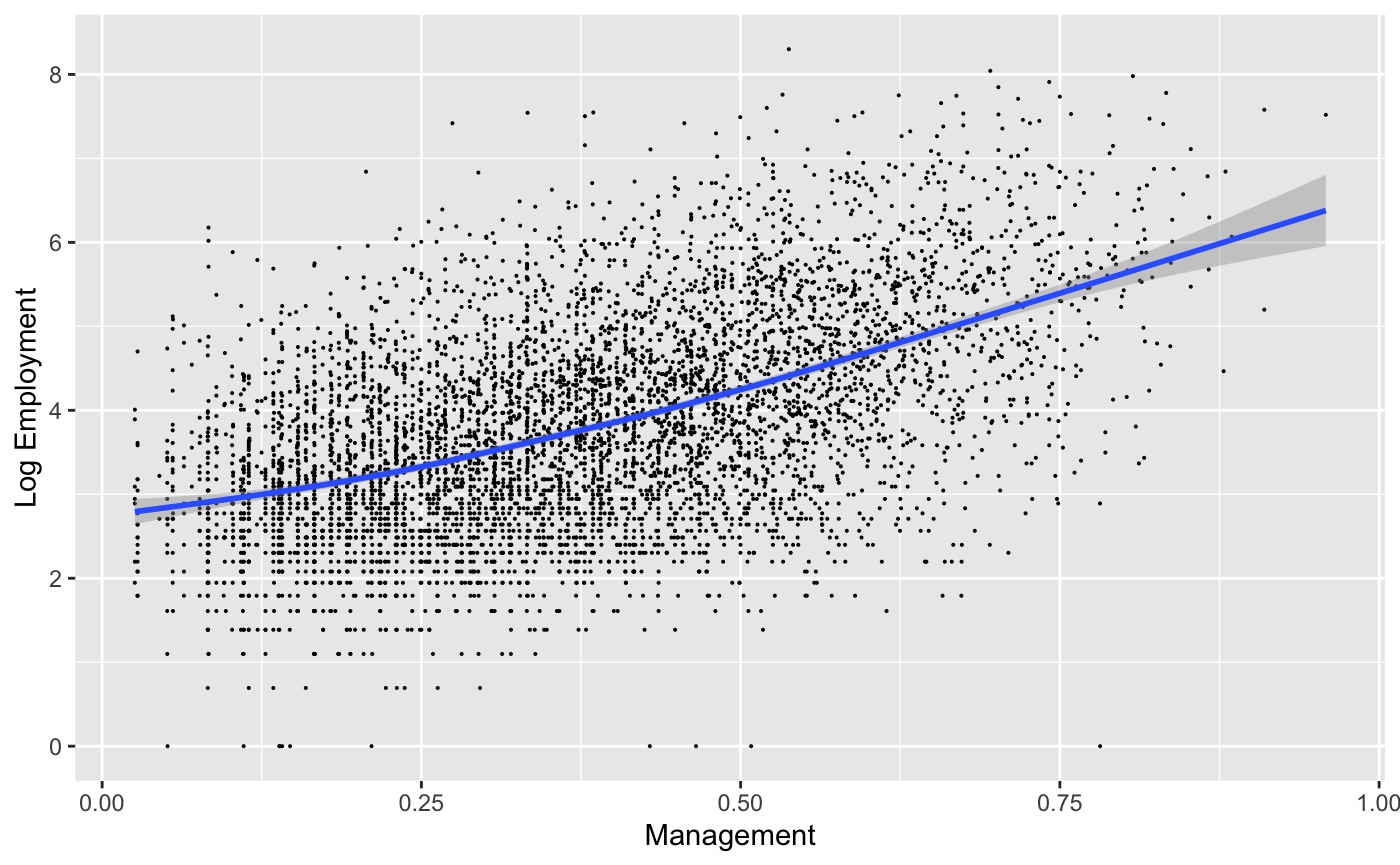
\includegraphics[scale = 0.28]{Images/Firm_size_Employment.jpg}
\end{figure}



\begin{table}
\caption{Firm Management Scores and Performance (1)}
\begin{center}
\begin{small}
\begin{tabular}{l c c c c c c c c c}
\hline
 & \multicolumn{3}{c}{Ln(Output/Emp)} & \multicolumn{3}{c}{Ln(Sales/Emp)} & \multicolumn{3}{c}{Profit/Sales} \\
\cline{2-4} \cline{5-7} \cline{8-10}
 & 1 & 2 & 3 & 4 & 5 & 6 & 7 & 8 & 9 \\
\hline
Management     & $0.24^{***}$ & $0.24^{***}$ & $0.25^{***}$ & $0.25^{***}$ & $0.25^{***}$ & $0.26^{***}$ & $-0.01$      & $0.02$       & $0.01$       \\
               & $(0.03)$     & $(0.03)$     & $(0.04)$     & $(0.03)$     & $(0.04)$     & $(0.04)$     & $(0.06)$     & $(0.06)$     & $(0.06)$     \\
Ln(Cap/Emp)    & $0.05^{***}$ & $0.05^{***}$ & $0.05^{***}$ & $0.05^{***}$ & $0.05^{***}$ & $0.05^{***}$ & $-0.01$      & $-0.01$      & $-0.01$      \\
               & $(0.01)$     & $(0.01)$     & $(0.01)$     & $(0.01)$     & $(0.01)$     & $(0.01)$     & $(0.01)$     & $(0.01)$     & $(0.01)$     \\
Ln(Input/Emp)  & $0.67^{***}$ & $0.68^{***}$ & $0.68^{***}$ & $0.66^{***}$ & $0.67^{***}$ & $0.67^{***}$ & $0.12^{***}$ & $0.10^{***}$ & $0.10^{***}$ \\
               & $(0.01)$     & $(0.01)$     & $(0.01)$     & $(0.01)$     & $(0.01)$     & $(0.01)$     & $(0.03)$     & $(0.03)$     & $(0.03)$     \\
Ln(Employment) & $0.05^{***}$ & $0.05^{***}$ & $0.05^{***}$ & $0.04^{***}$ & $0.04^{***}$ & $0.05^{***}$ & $0.01$       & $0.01$       & $0.01$       \\
               & $(0.01)$     & $(0.01)$     & $(0.01)$     & $(0.01)$     & $(0.01)$     & $(0.01)$     & $(0.01)$     & $(0.01)$     & $(0.01)$     \\
Degree         & $0.23^{***}$ & $0.47^{***}$ & $0.46^{***}$ & $0.27^{***}$ & $0.54^{***}$ & $0.52^{***}$ & $-0.07$      & $-0.16$      & $-0.15$      \\
               & $(0.06)$     & $(0.06)$     & $(0.06)$     & $(0.06)$     & $(0.06)$     & $(0.06)$     & $(0.11)$     & $(0.12)$     & $(0.12)$     \\
\hline
R$^2$          & $0.87$       & $0.86$       & $0.86$       & $0.87$       & $0.85$       & $0.85$       & $0.07$       & $0.03$       & $0.03$       \\
Adj. R$^2$     & $0.87$       & $0.86$       & $0.86$       & $0.86$       & $0.85$       & $0.85$       & $0.05$       & $0.03$       & $0.03$       \\
Num. obs.      & $5988$       & $5988$       & $5988$       & $5988$       & $5988$       & $5988$       & $5988$       & $5988$       & $5988$       \\
\hline
\multicolumn{10}{l}{\tiny{\parbox{0.95\linewidth}{\vspace{3pt}$^{***}p<0.001$; $^{**}p<0.01$; $^{*}p<0.05$. \\OLS coefficients with standard errors in parentheses (clustered at firm level). The management score is the unweighted average of the score for each of the 16 questions, where each question is first normalized to be on a 0–1 scale. The sample is all EDIT observations with at least 11 non-missing responses to management questions and a successful match to EAM, which have positive value added, positive employment, and positive imputed capital. The columns 1-3 mean the models with Industry Fixed Effects, Location Fixed Effects and no Fixed Effects, respectively.This also applies for columns 4-6 and 7-9. The regressions include clustered standard errors by CIIU4 and region, depending on the fixed effect applied}}}
\end{tabular}
\end{small}
\label{table:coefficients}
\end{center}
\end{table}

\begin{table}
\caption{Firm Management Scores and Performance (2)}
\begin{center}
\begin{small}
\begin{tabular}{l c c c c c c c c c}
\hline
 & \multicolumn{3}{c}{Log(VA/Emp)} & \multicolumn{3}{c}{Log(1+IP Registers)} & \multicolumn{3}{c}{Log(1+RDi/Emp)} \\
\cline{2-4} \cline{5-7} \cline{8-10}
 & 1 & 2 & 3 & 4 & 5 & 6 & 7 & 8 & 9 \\
\hline
Management     & $0.64^{***}$ & $0.69^{***}$ & $0.71^{***}$ & $0.51^{***}$ & $0.55^{***}$ & $0.55^{***}$ & $2.94^{***}$ & $2.93^{***}$ & $3.07^{***}$ \\
               & $(0.09)$     & $(0.09)$     & $(0.09)$     & $(0.12)$     & $(0.12)$     & $(0.12)$     & $(0.57)$     & $(0.57)$     & $(0.56)$     \\
Ln(Cap/Emp)    & $0.21^{***}$ & $0.24^{***}$ & $0.24^{***}$ & $0.09^{***}$ & $0.09^{***}$ & $0.09^{***}$ & $0.19^{*}$   & $0.33^{***}$ & $0.33^{***}$ \\
               & $(0.01)$     & $(0.01)$     & $(0.01)$     & $(0.02)$     & $(0.02)$     & $(0.01)$     & $(0.08)$     & $(0.07)$     & $(0.07)$     \\
Ln(Employment) & $0.18^{***}$ & $0.17^{***}$ & $0.18^{***}$ & $0.33^{***}$ & $0.32^{***}$ & $0.32^{***}$ & $0.11$       & $0.07$       & $0.09$       \\
               & $(0.01)$     & $(0.01)$     & $(0.01)$     & $(0.02)$     & $(0.02)$     & $(0.02)$     & $(0.08)$     & $(0.08)$     & $(0.08)$     \\
Degree         & $0.89^{***}$ & $1.39^{***}$ & $1.39^{***}$ & $1.06^{***}$ & $2.11^{***}$ & $2.11^{***}$ & $1.54$       & $2.79^{***}$ & $2.64^{**}$  \\
               & $(0.15)$     & $(0.15)$     & $(0.14)$     & $(0.20)$     & $(0.22)$     & $(0.22)$     & $(0.95)$     & $(0.82)$     & $(0.81)$     \\
\hline
R$^2$          & $0.33$       & $0.28$       & $0.27$       & $0.42$       & $0.29$       & $0.28$       & $0.17$       & $0.08$       & $0.07$       \\
Adj. R$^2$     & $0.31$       & $0.28$       & $0.27$       & $0.39$       & $0.28$       & $0.28$       & $0.11$       & $0.07$       & $0.07$       \\
Num. obs.      & $5988$       & $5988$       & $5988$       & $2534$       & $2534$       & $2534$       & $1749$       & $1749$       & $1749$       \\
\hline
\multicolumn{10}{l}{\tiny{\parbox{0.95\linewidth}{\vspace{3pt}$^{***}p<0.001$; $^{**}p<0.01$; $^{*}p<0.05$. \\OLS coefficients with standard errors in parentheses. The management score is the unweighted average of the score for each of the 16 questions, where each question is first normalized to be on a 0–1 scale. The sample is all EDIT observations with at least 11 non-missing responses to management questions and a successful match to EAM, which have positive value added, positive employment, and positive imputed capital. The columns 1-3 mean the models with Industry Fixed Effects, Location Fixed Effects and no Fixed Effects, respectively.This also applies for columns 4-6 and 7-9.The regressions include clustered standard errors by CIIU4 and region, depending on the fixed effect applied}}}
\end{tabular}
\end{small}
\label{table:coefficients}
\end{center}
\end{table}


\begin{table}
\caption{Drivers of Productivity Variation}
\begin{center}
\begin{normalsize}
\begin{tabular}{l c c c c}
\hline
 & \multicolumn{4}{c}{Log(VA/Emp)} \\
\cline{2-5}
 & 1 & 2 & 3 & 4 \\
\hline
Management & $1.950^{***}$ & $1.687^{***}$ & $1.694^{***}$ & $1.652^{***}$ \\
           & $(0.080)$     & $(0.084)$     & $(0.084)$     & $(0.083)$     \\
RDi        &               & $0.044^{***}$ & $0.043^{***}$ & $0.038^{***}$ \\
           &               & $(0.005)$     & $(0.004)$     & $(0.004)$     \\
ICT/Emp    &               &               & $0.000$       & $0.000$       \\
           &               &               & $(0.000)$     & $(0.000)$     \\
Degree     &               &               &               & $1.517^{***}$ \\
           &               &               &               & $(0.148)$     \\
\hline
R$^2$      & $0.101$       & $0.115$       & $0.116$       & $0.139$       \\
Adj. R$^2$ & $0.100$       & $0.115$       & $0.116$       & $0.138$       \\
Num. obs.  & $6026$        & $6026$        & $6026$        & $6026$        \\
\hline
\multicolumn{5}{l}{\scriptsize{\parbox{1\linewidth}{\vspace{3pt}$^{***}p<0.001$; $^{**}p<0.01$; $^{*}p<0.05$. \\OLS coefficients with standard errors in parentheses.Dependent variable is firm level log(Value Added/Employment). Independent variables are Management score, RDi is measured as log(1+RDi intensity), where RDi intensity is the total domestic Research, Development and innovation expenditure in 2018 divided by total domestic employment, ICT/Emp is investment per worker (spending on information and communication technology hardware and software per employee), Degree is measured by the share of employees (managers and non-managers) with a college degree.Missing values have been replaced by zero for RDi and by means for the other variables. The regressions include standard errors clustered by firm}}}
\end{tabular}
\end{normalsize}
\label{table:coefficients}
\end{center}
\end{table}


\begin{table}
\caption{China Import Share and Management}
\begin{center}
\begin{normalsize}
\begin{tabular}{l c c}
\hline
 & \multicolumn{2}{c}{Management} \\
\cline{2-3}
 & 1 & 2 \\
\hline
China Import Share & $-0.097^{**}$ & $-0.031^{*}$  \\
                   & $(0.033)$     & $(0.015)$     \\
Ln(Cap/Emp)        &               & $0.013^{***}$ \\
                   &               & $(0.002)$     \\
Ln(Employment)     &               & $0.070^{***}$ \\
                   &               & $(0.003)$     \\
Degree             &               & $0.149^{***}$ \\
                   &               & $(0.022)$     \\
\hline
R$^2$              & $0.011$       & $0.300$       \\
Adj. R$^2$         & $0.011$       & $0.299$       \\
Num. obs.          & $5654$        & $5654$        \\
\hline
\multicolumn{3}{l}{\scriptsize{\parbox{0.9\linewidth}{\vspace{3pt}$^{***}p<0.001$; $^{**}p<0.01$; $^{*}p<0.05$. \\The China Import Share means imports from China / Total imports for each industry (4 digits CIIU rev4). This table uses this China Import Share without controls:column (1), and with full controls:column (2). We estimated the China Import Share according to the Import Origin published by DANE and matched them to the firm four digits CIIU4 codes.The regressions include clustered standard errors by four digits CIIU4 codes.}}}
\end{tabular}
\end{normalsize}
\label{table:coefficients}
\end{center}
\end{table}

\begin{table}
\caption{Dummies of trade outcomes and Management}
\begin{center}
\begin{normalsize}
\begin{tabular}{l c c c}
\hline
 & Dummy Exports & Dummy Imports & Dummy Trade \\
\hline
Management     & $0.192^{***}$ & $0.131^{***}$ & $0.211^{***}$ \\
               & $(0.035)$     & $(0.032)$     & $(0.035)$     \\
Ln(Cap/Emp)    & $0.043^{***}$ & $0.048^{***}$ & $0.046^{***}$ \\
               & $(0.005)$     & $(0.004)$     & $(0.005)$     \\
Ln(Employment) & $0.177^{***}$ & $0.147^{***}$ & $0.177^{***}$ \\
               & $(0.005)$     & $(0.005)$     & $(0.005)$     \\
Degree         & $0.380^{***}$ & $0.366^{***}$ & $0.382^{***}$ \\
               & $(0.054)$     & $(0.050)$     & $(0.056)$     \\
\hline
R$^2$          & $0.401$       & $0.384$       & $0.398$       \\
Adj. R$^2$     & $0.385$       & $0.368$       & $0.382$       \\
Num. obs.      & $5860$        & $5860$        & $5860$        \\
\hline
\multicolumn{4}{l}{\scriptsize{\parbox{1\linewidth}{\vspace{3pt}$^{***}p<0.001$; $^{**}p<0.01$; $^{*}p<0.05$. \\This table examines the relationship between export status (Dummy Exports = 1 if value of exported products>0 and 0 otherwise), import status (Dummy Import=1 if value of imported inputs>0 and 0 otherwise), trade status (Dummy Trade=1 if value of exports + imports>0 and 0 otherwise) and firm's management practices.It includes some controls: Ln(Cap/Emp), Ln(Employment) and the percent of staff with college degree. All regressions include fixed effects for firm location (department) and 4 digits - CIIU 4 (industry) and clustered standard errors by firm.}}}
\end{tabular}
\end{normalsize}
\label{table:coefficients}
\end{center}
\end{table}

\begin{table}
\caption{Extensive and Intensive Margins for Exporters - With Employment Dummies and Fixed Effects}
\begin{center}
\begin{small}
\begin{tabular}{l c c c c c c c c}
\hline
 & LnD & LnP & LnD-P & LnExp & LnExp/D & Ln Exp/P & Ln Exp/D-P & Ln TopD-P \\
\hline
Management   & $0.94^{***}$ & $0.92^{***}$ & $1.29^{***}$ & $1.82^{***}$ & $0.88^{***}$ & $0.89^{**}$  & $0.52^{*}$   & $1.44^{***}$ \\
             & $(0.15)$     & $(0.15)$     & $(0.20)$     & $(0.33)$     & $(0.25)$     & $(0.28)$     & $(0.23)$     & $(0.31)$     \\
Ln(Cap/Emp)  & $0.02$       & $-0.02$      & $-0.01$      & $0.19^{***}$ & $0.17^{***}$ & $0.21^{***}$ & $0.20^{***}$ & $0.21^{***}$ \\
             & $(0.02)$     & $(0.02)$     & $(0.03)$     & $(0.05)$     & $(0.04)$     & $(0.04)$     & $(0.03)$     & $(0.04)$     \\
Big=1        & $1.13^{***}$ & $1.07^{***}$ & $1.57^{***}$ & $2.80^{***}$ & $1.67^{***}$ & $1.74^{***}$ & $1.23^{***}$ & $2.32^{***}$ \\
             & $(0.08)$     & $(0.08)$     & $(0.11)$     & $(0.17)$     & $(0.12)$     & $(0.14)$     & $(0.12)$     & $(0.15)$     \\
Medium=1     & $0.44^{***}$ & $0.41^{***}$ & $0.62^{***}$ & $1.08^{***}$ & $0.64^{***}$ & $0.66^{***}$ & $0.46^{***}$ & $0.87^{***}$ \\
             & $(0.05)$     & $(0.05)$     & $(0.07)$     & $(0.12)$     & $(0.09)$     & $(0.10)$     & $(0.09)$     & $(0.11)$     \\
Degree       & $1.23^{***}$ & $1.32^{***}$ & $1.80^{***}$ & $1.33^{*}$   & $0.10$       & $0.01$       & $-0.47$      & $0.56$       \\
             & $(0.26)$     & $(0.26)$     & $(0.34)$     & $(0.52)$     & $(0.37)$     & $(0.44)$     & $(0.36)$     & $(0.47)$     \\
Ln(Wage/Emp) & $0.32^{***}$ & $0.34^{***}$ & $0.49^{***}$ & $0.85^{***}$ & $0.53^{***}$ & $0.51^{***}$ & $0.37^{***}$ & $0.69^{***}$ \\
             & $(0.06)$     & $(0.05)$     & $(0.07)$     & $(0.13)$     & $(0.10)$     & $(0.12)$     & $(0.10)$     & $(0.13)$     \\
\hline
R$^2$        & $0.37$       & $0.38$       & $0.38$       & $0.45$       & $0.39$       & $0.41$       & $0.38$       & $0.43$       \\
Adj. R$^2$   & $0.32$       & $0.34$       & $0.34$       & $0.41$       & $0.35$       & $0.37$       & $0.34$       & $0.38$       \\
Num. obs.    & $2044$       & $2044$       & $2044$       & $2044$       & $2044$       & $2044$       & $2044$       & $2044$       \\
\hline
\multicolumn{9}{l}{\tiny{\parbox{1\linewidth}{\vspace{3pt}$^{***}p<0.001$; $^{**}p<0.01$; $^{*}p<0.05$. \\This table examines the relationship between firms' management practices and the extensive and intensive margins of their exports. LnD:Log of destinations,LnP:Log of products by HS 6 digits,LnD-P: Log of pairs destination-products,LnExp: Log of Exports, LnExp/D: Log(Exports/Destinations,Ln Exp/P:Log(Exports/Products),Ln Exp/D-P:Log(Exports/pairs destination-products),Ln TopD-P:Log(exports in a firm's highest-revenue destination-product).The regressions include dummies employment as a control, where 50<medium<250 workers,big>250 and small<50 is excluded by collinearity. It also has standard errors clustered by firm.}}}
\end{tabular}
\end{small}
\label{table:coefficients}
\end{center}
\end{table}

\begin{table}
\caption{Extensive and Intensive Margins for all firms - With Employment Dummies and Fixed Effects}
\begin{center}
\begin{small}
\begin{tabular}{l c c c c c c c c}
\hline
 & Ln(1+D) & Ln(1+P) & Ln(1+DP) & Ln(1+E) & Ln(1+E/D) & Ln(1+E/P) & Ln(1+E/D-P) & Ln(1+TopDP) \\
\hline
Manag      & $0.80^{***}$ & $0.76^{***}$ & $1.09^{***}$ & $4.82^{***}$ & $4.07^{***}$ & $4.12^{***}$ & $3.76^{***}$ & $4.49^{***}$ \\
           & $(0.07)$     & $(0.07)$     & $(0.10)$     & $(0.46)$     & $(0.41)$     & $(0.41)$     & $(0.38)$     & $(0.43)$     \\
Ln(C/E)    & $0.04^{***}$ & $0.02^{*}$   & $0.04^{**}$  & $0.28^{***}$ & $0.25^{***}$ & $0.26^{***}$ & $0.24^{***}$ & $0.27^{***}$ \\
           & $(0.01)$     & $(0.01)$     & $(0.01)$     & $(0.06)$     & $(0.05)$     & $(0.05)$     & $(0.05)$     & $(0.06)$     \\
Big=1      & $1.13^{***}$ & $1.14^{***}$ & $1.65^{***}$ & $6.42^{***}$ & $5.31^{***}$ & $5.32^{***}$ & $4.77^{***}$ & $5.90^{***}$ \\
           & $(0.06)$     & $(0.06)$     & $(0.08)$     & $(0.30)$     & $(0.26)$     & $(0.26)$     & $(0.24)$     & $(0.28)$     \\
Med=1      & $0.43^{***}$ & $0.46^{***}$ & $0.63^{***}$ & $3.08^{***}$ & $2.70^{***}$ & $2.68^{***}$ & $2.49^{***}$ & $2.88^{***}$ \\
           & $(0.03)$     & $(0.03)$     & $(0.04)$     & $(0.17)$     & $(0.15)$     & $(0.15)$     & $(0.14)$     & $(0.16)$     \\
Degree     & $0.66^{***}$ & $0.72^{***}$ & $1.01^{***}$ & $3.33^{***}$ & $2.68^{***}$ & $2.61^{***}$ & $2.32^{***}$ & $2.95^{***}$ \\
           & $(0.11)$     & $(0.12)$     & $(0.16)$     & $(0.70)$     & $(0.62)$     & $(0.62)$     & $(0.58)$     & $(0.66)$     \\
Ln(W/E)    & $0.27^{***}$ & $0.28^{***}$ & $0.40^{***}$ & $1.59^{***}$ & $1.33^{***}$ & $1.32^{***}$ & $1.19^{***}$ & $1.45^{***}$ \\
           & $(0.03)$     & $(0.03)$     & $(0.04)$     & $(0.19)$     & $(0.17)$     & $(0.17)$     & $(0.16)$     & $(0.18)$     \\
\hline
R$^2$      & $0.39$       & $0.36$       & $0.38$       & $0.37$       & $0.35$       & $0.36$       & $0.35$       & $0.37$       \\
Adj. R$^2$ & $0.37$       & $0.34$       & $0.36$       & $0.36$       & $0.34$       & $0.34$       & $0.33$       & $0.35$       \\
Num. obs.  & $5835$       & $5835$       & $5835$       & $5835$       & $5835$       & $5835$       & $5835$       & $5835$       \\
\hline
\multicolumn{9}{l}{\tiny{\parbox{1\linewidth}{\vspace{3pt}$^{***}p<0.001$; $^{**}p<0.01$; $^{*}p<0.05$. \\This table examines the relationship between firms' management practices and the extensive and intensive margins for the entire sample applying the transformation (1 + variable). D:destinations,P:products by HS 6 digits,DP:pairs destination-products,E:Exports,E/D:Exports/Destinations,E/P:Exports/Products,E/D-P:Exports/pairs destination-products,TopD-P:exports in a firm's highest-revenue destination-product.The regressions include dummies employment as a control, where 50<medium<250 workers,big>250 and small<50 is excluded by collinearity. It also has standard errors clustered by firm.}}}
\end{tabular}
\end{small}
\label{table:coefficients}
\end{center}
\end{table}


\begin{table}
\caption{Extensive and Intensive Margins for Non-Complex Products}
\begin{center}
\begin{normalsize}
\begin{tabular}{l c c c c c c c c}
\hline
 & LnD & LnP & LnD-P & LnExp & LnExp/D & Ln Exp/P & Ln Exp/D-P & Ln TopD-P \\
\hline
Management   & $0.62^{**}$  & $0.79^{***}$ & $1.03^{***}$ & $1.02^{*}$   & $0.39$       & $0.23$       & $-0.01$      & $0.71$       \\
             & $(0.21)$     & $(0.21)$     & $(0.27)$     & $(0.50)$     & $(0.39)$     & $(0.44)$     & $(0.37)$     & $(0.47)$     \\
Ln(Cap/Emp)  & $0.01$       & $-0.05$      & $-0.04$      & $0.20^{**}$  & $0.19^{***}$ & $0.25^{***}$ & $0.24^{***}$ & $0.24^{***}$ \\
             & $(0.03)$     & $(0.03)$     & $(0.04)$     & $(0.06)$     & $(0.05)$     & $(0.06)$     & $(0.05)$     & $(0.06)$     \\
Big=1        & $1.33^{***}$ & $1.15^{***}$ & $1.79^{***}$ & $3.08^{***}$ & $1.75^{***}$ & $1.93^{***}$ & $1.29^{***}$ & $2.51^{***}$ \\
             & $(0.11)$     & $(0.11)$     & $(0.15)$     & $(0.25)$     & $(0.20)$     & $(0.22)$     & $(0.20)$     & $(0.24)$     \\
Medium=1     & $0.48^{***}$ & $0.34^{***}$ & $0.63^{***}$ & $1.05^{***}$ & $0.57^{***}$ & $0.71^{***}$ & $0.42^{**}$  & $0.81^{***}$ \\
             & $(0.08)$     & $(0.07)$     & $(0.10)$     & $(0.19)$     & $(0.15)$     & $(0.17)$     & $(0.14)$     & $(0.18)$     \\
Degree       & $1.32^{**}$  & $0.95^{*}$   & $1.61^{**}$  & $0.93$       & $-0.39$      & $-0.03$      & $-0.69$      & $0.14$       \\
             & $(0.43)$     & $(0.43)$     & $(0.58)$     & $(0.81)$     & $(0.60)$     & $(0.75)$     & $(0.65)$     & $(0.77)$     \\
Ln(Wage/Emp) & $0.32^{***}$ & $0.34^{***}$ & $0.49^{***}$ & $0.93^{***}$ & $0.61^{***}$ & $0.59^{***}$ & $0.43^{**}$  & $0.74^{***}$ \\
             & $(0.08)$     & $(0.07)$     & $(0.09)$     & $(0.19)$     & $(0.15)$     & $(0.17)$     & $(0.14)$     & $(0.18)$     \\
\hline
R$^2$        & $0.42$       & $0.47$       & $0.46$       & $0.48$       & $0.42$       & $0.45$       & $0.42$       & $0.46$       \\
Adj. R$^2$   & $0.34$       & $0.40$       & $0.39$       & $0.42$       & $0.34$       & $0.38$       & $0.35$       & $0.39$       \\
Num. obs.    & $1011$       & $1011$       & $1011$       & $1011$       & $1011$       & $1011$       & $1011$       & $1011$       \\
\hline
\multicolumn{9}{l}{\scriptsize{\parbox{1\linewidth}{\vspace{3pt}$^{***}p<0.001$; $^{**}p<0.01$; $^{*}p<0.05$. \\This table examines the relationship between firms' management practices and the extensive and intensive margins of their exports, filtering data for complex products according to product complexity ranking from Atlas of Economic Complexity. This table uses a sub-sample, where the products have a complexity index lower than its median of the entire sample. The complex index is calculated at HS 4digits and matched with the firm's products. LnD:Log of destinations,LnP:Log of products by HS 6 digits,LnD-P: Log of pairs destination-products,LnExp: Log of Exports, LnExp/D: Log(Exports/Destinations,Ln Exp/P:Log(Exports/Products),Ln Exp/D-P:Log(Exports/pairs destination-products),Ln TopD-P:Log(exports in a firm's highest-revenue destination-product).The regressions include dummies employment as a control, where 50<medium<250 workers,big>250 and small<50 is excluded by collinearity. It also has standard errors clustered by firm.}}}
\end{tabular}
\end{normalsize}
\label{table:coefficients}
\end{center}
\end{table}

\begin{table}
\caption{Extensive and Intensive Margins for Complex Products}
\begin{center}
\begin{normalsize}
\begin{tabular}{l c c c c c c c c}
\hline
 & LnD & LnP & LnD-P & LnExp & LnExp/D & Ln Exp/P & Ln Exp/D-P & Ln TopD-P \\
\hline
Management   & $1.14^{***}$ & $0.99^{***}$ & $1.42^{***}$ & $2.38^{***}$ & $1.25^{***}$ & $1.39^{***}$ & $0.97^{**}$  & $2.00^{***}$ \\
             & $(0.22)$     & $(0.23)$     & $(0.30)$     & $(0.48)$     & $(0.34)$     & $(0.38)$     & $(0.31)$     & $(0.42)$     \\
Ln(Cap/Emp)  & $0.04$       & $0.03$       & $0.04$       & $0.21^{**}$  & $0.17^{**}$  & $0.19^{**}$  & $0.18^{***}$ & $0.21^{**}$  \\
             & $(0.04)$     & $(0.03)$     & $(0.05)$     & $(0.08)$     & $(0.05)$     & $(0.07)$     & $(0.05)$     & $(0.07)$     \\
Big=1        & $0.99^{***}$ & $1.03^{***}$ & $1.44^{***}$ & $2.59^{***}$ & $1.60^{***}$ & $1.56^{***}$ & $1.15^{***}$ & $2.16^{***}$ \\
             & $(0.12)$     & $(0.12)$     & $(0.16)$     & $(0.25)$     & $(0.17)$     & $(0.21)$     & $(0.16)$     & $(0.22)$     \\
Medium=1     & $0.40^{***}$ & $0.47^{***}$ & $0.62^{***}$ & $1.07^{***}$ & $0.67^{***}$ & $0.60^{***}$ & $0.45^{***}$ & $0.88^{***}$ \\
             & $(0.08)$     & $(0.08)$     & $(0.11)$     & $(0.17)$     & $(0.12)$     & $(0.14)$     & $(0.11)$     & $(0.15)$     \\
Degree       & $1.13^{**}$  & $1.39^{***}$ & $1.78^{***}$ & $1.33$       & $0.21$       & $-0.06$      & $-0.45$      & $0.63$       \\
             & $(0.35)$     & $(0.36)$     & $(0.47)$     & $(0.74)$     & $(0.52)$     & $(0.60)$     & $(0.48)$     & $(0.65)$     \\
Ln(Wage/Emp) & $0.33^{***}$ & $0.32^{***}$ & $0.47^{***}$ & $0.75^{***}$ & $0.42^{**}$  & $0.43^{*}$   & $0.28^{*}$   & $0.59^{**}$  \\
             & $(0.10)$     & $(0.09)$     & $(0.13)$     & $(0.20)$     & $(0.14)$     & $(0.17)$     & $(0.14)$     & $(0.18)$     \\
\hline
R$^2$        & $0.39$       & $0.38$       & $0.40$       & $0.47$       & $0.43$       & $0.42$       & $0.39$       & $0.46$       \\
Adj. R$^2$   & $0.31$       & $0.30$       & $0.32$       & $0.40$       & $0.36$       & $0.34$       & $0.31$       & $0.39$       \\
Num. obs.    & $1010$       & $1010$       & $1010$       & $1010$       & $1010$       & $1010$       & $1010$       & $1010$       \\
\hline
\multicolumn{9}{l}{\scriptsize{\parbox{1\linewidth}{\vspace{3pt}$^{***}p<0.001$; $^{**}p<0.01$; $^{*}p<0.05$. \\This table examines the relationship between firms' management practices and the extensive and intensive margins of their exports, filtering data for complex products according to product complexity ranking from Atlas of Economic Complexity. This table uses a sub-sample, where the products have a product complexity index greater than its median of the entire sample . he complex index is calculated at HS 4digits and matched with the firm's products. LnD:Log of destinations,LnP:Log of products by HS 6 digits,LnD-P: Log of pairs destination-products,LnExp: Log of Exports, LnExp/D: Log(Exports/Destinations,Ln Exp/P:Log(Exports/Products),Ln Exp/D-P:Log(Exports/pairs destination-products),Ln TopD-P:Log(exports in a firm's highest-revenue destination-product).The regressions include dummies employment as a control, where 50<medium<250 workers,big>250 and small<50 is excluded by collinearity. It also has standard errors clustered by firm.}}}
\end{tabular}
\end{normalsize}
\label{table:coefficients}
\end{center}
\end{table}

\begin{table}
\caption{Gravity Equation - Exporters}
\begin{center}
\begin{normalsize}
\begin{tabular}{l c c c c}
\hline
 & \multicolumn{4}{c}{Ln Exports} \\
\cline{2-5}
 & 1 & 2 & 3 & 4 \\
\hline
Management              & $0.65^{*}$   & $0.82^{**}$   & $4.14^{*}$   & $5.13^{*}$   \\
                        & $(0.26)$     & $(0.27)$      & $(1.82)$     & $(2.49)$     \\
Ln(Cap/Emp)             & $0.18^{***}$ & $0.17^{***}$  & $0.16^{***}$ & $0.16^{***}$ \\
                        & $(0.04)$     & $(0.04)$      & $(0.04)$     & $(0.04)$     \\
Big=1                   & $0.90^{***}$ & $1.13^{***}$  & $1.13^{***}$ & $1.13^{***}$ \\
                        & $(0.12)$     & $(0.13)$      & $(0.13)$     & $(0.12)$     \\
Medium=1                & $0.31^{**}$  & $0.39^{***}$  & $0.38^{***}$ & $0.38^{***}$ \\
                        & $(0.10)$     & $(0.10)$      & $(0.10)$     & $(0.10)$     \\
Degree                  & $0.11$       & $0.66$        & $0.67$       & $0.67$       \\
                        & $(0.49)$     & $(0.49)$      & $(0.49)$     & $(0.49)$     \\
Ln(Wage/Emp)            & $0.09$       & $0.14$        & $0.15$       & $0.15$       \\
                        & $(0.12)$     & $(0.12)$      & $(0.12)$     & $(0.12)$     \\
Ln (GDP of destination) &              & $0.28^{***}$  & $0.28^{***}$ & $0.31^{***}$ \\
                        &              & $(0.02)$      & $(0.02)$     & $(0.05)$     \\
Ln Distance             &              & $-0.54^{***}$ & $-0.31^{*}$  & $-0.35^{*}$  \\
                        &              & $(0.06)$      & $(0.14)$     & $(0.16)$     \\
Common Language=1       &              & $0.64^{***}$  & $0.64^{***}$ & $0.64^{***}$ \\
                        &              & $(0.08)$      & $(0.08)$     & $(0.08)$     \\
Contiguous=1            &              & $0.26^{***}$  & $0.28^{***}$ & $0.28^{***}$ \\
                        &              & $(0.06)$      & $(0.06)$     & $(0.06)$     \\
Inter(Manag*Dist)       &              &               & $-0.42$      & $-0.34$      \\
                        &              &               & $(0.24)$     & $(0.27)$     \\
Inter(Manag*Produc)     &              &               &              & $-0.06$      \\
                        &              &               &              & $(0.10)$     \\
\hline
R$^2$                   & $0.14$       & $0.20$        & $0.20$       & $0.20$       \\
Adj. R$^2$              & $0.13$       & $0.19$        & $0.19$       & $0.19$       \\
Num. obs.               & $14502$      & $14502$       & $14502$      & $14502$      \\
\hline
\multicolumn{5}{l}{\scriptsize{\parbox{1\linewidth}{\vspace{3pt}$^{***}p<0.001$; $^{**}p<0.01$; $^{*}p<0.05$. \\ This table examines the relationship between exports revenues of each country and firm's management practices. The column 1 has controls at firm level: capital per employees, dummies of size measured by employment(Big=1,Medium=1), the share of staff with college degree and the average wage.This table uses dummies of size (medium greater or equal than 50 and less than 250 workers,big greater than 250; small less than 50 is excluded by collinearity).From column 2 to column 4, we adds controls at country level: log of GDP of destination country, log of distance between the destination country and Colombia and dummies of common language and geographic contiguity.The regressions include fixed effects for CIIU4 and location and standard errors clustered by firm}}}
\end{tabular}
\end{normalsize}
\label{table:coefficients}
\end{center}
\end{table}

\begin{table}
\caption{Gravity Equation-all firms}
\begin{center}
\begin{normalsize}
\begin{tabular}{l c c c c}
\hline
 & \multicolumn{4}{c}{Ln (1+Exports)} \\
\cline{2-5}
 & 1 & 2 & 3 & 4 \\
\hline
Management              & $1.82^{***}$ & $1.72^{***}$  & $17.33^{***}$ & $14.85^{***}$ \\
                        & $(0.32)$     & $(0.30)$      & $(2.25)$      & $(2.60)$      \\
Ln(Cap/Emp)             & $0.28^{***}$ & $0.29^{***}$  & $0.29^{***}$  & $0.29^{***}$  \\
                        & $(0.05)$     & $(0.05)$      & $(0.05)$      & $(0.05)$      \\
Big=1                   & $2.07^{***}$ & $1.99^{***}$  & $1.92^{***}$  & $1.91^{***}$  \\
                        & $(0.16)$     & $(0.16)$      & $(0.16)$      & $(0.16)$      \\
Medium=1                & $1.55^{***}$ & $1.49^{***}$  & $1.40^{***}$  & $1.40^{***}$  \\
                        & $(0.14)$     & $(0.14)$      & $(0.13)$      & $(0.13)$      \\
Degree                  & $0.13$       & $-0.12$       & $-0.26$       & $-0.28$       \\
                        & $(0.58)$     & $(0.57)$      & $(0.59)$      & $(0.59)$      \\
Ln(Wage/Emp)            & $0.35^{*}$   & $0.34^{**}$   & $0.35^{**}$   & $0.34^{**}$   \\
                        & $(0.14)$     & $(0.13)$      & $(0.13)$      & $(0.13)$      \\
Ln (GDP of destination) &              & $0.18^{***}$  & $0.16^{***}$  & $0.08$        \\
                        &              & $(0.02)$      & $(0.02)$      & $(0.05)$      \\
Ln Distance             &              & $-0.07$       & $1.07^{***}$  & $1.19^{***}$  \\
                        &              & $(0.06)$      & $(0.20)$      & $(0.21)$      \\
Common Language=1       &              & $-0.03$       & $-0.03$       & $-0.05$       \\
                        &              & $(0.09)$      & $(0.09)$      & $(0.09)$      \\
Contiguous=1            &              & $-0.50^{***}$ & $-0.43^{***}$ & $-0.43^{***}$ \\
                        &              & $(0.08)$      & $(0.08)$      & $(0.08)$      \\
Inter(Manag*Dist)       &              &               & $-2.04^{***}$ & $-2.26^{***}$ \\
                        &              &               & $(0.30)$      & $(0.33)$      \\
Inter(Manag*Produc)     &              &               &               & $0.16$        \\
                        &              &               &               & $(0.09)$      \\
\hline
R$^2$                   & $0.18$       & $0.19$        & $0.20$        & $0.20$        \\
Adj. R$^2$              & $0.18$       & $0.19$        & $0.20$        & $0.20$        \\
Num. obs.               & $67134$      & $67134$       & $67134$       & $67134$       \\
\hline
\multicolumn{5}{l}{\scriptsize{\parbox{1\linewidth}{\vspace{3pt}$^{***}p<0.001$; $^{**}p<0.01$; $^{*}p<0.05$. \\ This table examines the relationship between exports revenues of each country and firm's management practices for all firms (exporters and no exporters) by using Ln (1+Exp). The column 1 has controls at firm level: capital per employees, dummies of size measured by employment(Big=1,Medium=1), the share of staff with college degree and the average wage.This table uses dummies of size (medium greater or equal than 50 and less than 250 workers,big greater than 250; small less than 50 is excluded by collinearity). From column 2 to column 4, we adds controls at country level: log of GDP of destination country, log of distance between the destination country and Colombia and dummies of common language and geographic contiguity. For companies that do not export and do not have a destination country, we attribute Ecuador since it is the mode. We use the Ecuador's information to fulfill the GDP of destination and distance, common language and contiguity. The regressions include fixed effects for CIIU4 and location and standard errors clustered by firm}}}
\end{tabular}
\end{normalsize}
\label{table:coefficients}
\end{center}
\end{table}

\end{document}
